\documentclass{beamer}

\newenvironment{tightcenter}{%
  \setlength\topsep{0pt}
  \setlength\parskip{0pt}
  \begin{center}
}{%
  \end{center}
}

\mode<presentation>
{
  \usetheme{Copenhagen}
  %%\usecolortheme[RGB={173,222,25}]{structure}
  \usecolortheme[RGB={255,0,0}]{structure}
  \setbeamertemplate{items}[circle]
  \setbeamercovered{transparent}
}

\usepackage[polish]{babel}
\usepackage{chessfss}
\usepackage{hyperref}
\usepackage{qtree}
\usepackage{mathtools}
\usepackage{dirtytalk}
\usepackage{epigraph}
\usepackage{textgreek}
\usepackage[utf8]{inputenc}
\usepackage{times}
\usepackage[T1]{fontenc}
\usepackage{tikz}
\usepackage{csquotes}
\usepackage{amsmath}
\usepackage{fancyvrb}
\usepackage{ulem}
\usepackage{adjustbox}

\newenvironment{Snippet}{\Verbatim[samepage=true]}{\endVerbatim}

\title{\textbf{Kwadrans o Monadach}}

\author{Panicz Maciej Godek}

\institute{
  \tiny{\href{mailto:godek.maciek@gmail.com}{\textbf{godek.maciek@gmail.com}}} \\
  \normalsize{\url{https://github.com/panicz/writings/tree/master/talks/jug/kwadrans}}
}

\date{\textbf{JUG Trójmiasto}, 19.10.2023}

\begin{document}

\begin{frame}
  \titlepage
\end{frame}

\begin{frame}{Agenda}
  \begin{itemize}
    \pause \item koncepcja monady
    \pause \item problemy z Haskellem
    \pause \item piramida zagłady (z lukrem)
    \pause \item utyskiwania
  \end{itemize}
\end{frame}

\begin{frame}{Programowanie bezpunktowe}
  Odwrotność pierwiastka kwadratowego \\ \pause
  \texttt{isqrt x = 1/(sqrt x)} \\ \pause
  bezpunktowo: \\ \pause
  \texttt{isqrt = (1/) .\ sqrt} \\ \pause
  gdzie
  \texttt{(f .\ g) x = f (g x)} \\ \pause
  w JS: \\
  \texttt{function compose(f, g) \{ \\
    \ \ return function(x) \{ \\
    \ \ \ \ return f(g(x)); \\
    \ \ \}; \\
    \}}  
\end{frame}

\begin{frame}{Operator kompozycji}
  Typ operatora kompozycji: \\ \pause
  \texttt{(.) :: (b -> c) -> (a -> b) -> (a -> c)} \\ \pause
  wygląda trochę dziwacznie, ale jeżeli zdefiniujemy \\
  \texttt{(g | f) x = f (g x)} \\ \pause
  typem ``odwróconej kompozycji'' jest \\ \pause
  \texttt{(|) :: (a -> b) -> (b -> c) -> (a -> c)} \\ \pause
  vide potoki w UNIXie \\ \pause
  albo ``wujek kolegi mojego brata'' vs.\ ``mojego brata kolegi wujek'' \\ \pause
  albo \texttt{f(g(x))} vs.\ \texttt{x->getG()->getF()} \\ \pause
  czaicie rozumiecie
\end{frame}

\begin{frame}{Operator kompozycji}
  Własności operatora kompozycji: \pause
  \begin{itemize}
  \item łączny: \texttt{f .\ (g .\ h) = (f .\ g) .\ h} \\ \pause
    tak jak: \texttt{x + (y + z) = (x + y) + z} \\ \pause
    albo o: \texttt{x * (y * z) = (x * y) * z} \pause
  \item posiada element neutralny \texttt{id}: \\ \pause
    \texttt{f .\ id = id .\ f = f} \\ \pause
    tak jak: \texttt{x + 0 = 0 + x = x} \\ \pause
    albo: \texttt{x * 1 = 1 * x = x} \pause
  \end{itemize}
  gdzie funkcja tożsamościowa jest zdeiniowana jako\\
  \texttt{id x = x} \\ \pause
  \texttt{function id(x) \{ return x; \}}
\end{frame}


\begin{frame}{Och, ta matematyka}
  Matematycy nazywają operator łączny z elementem neutralnym \textit{monoidem}
  (albo \textit{półgrupą z jedynką}). \\ \pause
  A teraz wyobraźmy sobie takie uogólnienie operatora kompozycji: \\ \pause
  \texttt{<|$_m$ ::\ (b -> $m$ c) -> (a -> $m$ b) -> (a -> $m$ c)} \\ \pause
  Na przykład: \\
  \texttt{class WithLog<T> \{ \\
    \ \ public T value; \\
    \ \ public String log; \\
    \}} \\ \pause
  \texttt{(f <|$_\mathtt{WithLog}$ g) a = \\
    \ \ WithLog b = g(a); \\
    \ \ WithLog c = f(b.value); \\
    \ \ return WithLog(value = c.value, log = b.log + c.log); }
\end{frame}

\begin{frame}{Uogólnienie operatora identyczności}
  \texttt{id$_\mathtt{WithLog}$ x = WithLog(value = x, log = '''')} \\ \pause
  Trójkę \texttt{($m$, <|$_m$, id$_m$)} nazywamy \textit{monadą}. \\ \pause
  Na przykład \texttt{(WithLog, <|$_\mathtt{WithLog}$, id$_\mathtt{WithLog}$)}
  jest monadą. \\ \pause
  Inne popularne przykłady: \texttt{Optional}, \texttt{List}.

   %% \texttt{(f <|$_\mathtt{List}$ g) a = \\
   %%  \ \ List b = f(a); \\
   %%  \ \ List result = new LinkedList(); \\
   %%  \ \ for (Object x : b) \{ \\
   %%  \ \ \ \ result.addAll(g(x)); \\
   %%  \ \ \} \\
   %%  \ \ return result;}

\end{frame}

\begin{frame}{Ale dlaczego?}
  \pause
  Problem Haskella: leniwa ewaluacja. \\ \pause
  Rozwiązanie: ``system wejścia-wyjścia oparty na monadach'' \\ \pause
  Ale co to znaczy?!
\end{frame}

\begin{frame}{Strategie ewaluacji}
  \texttt{square x = x * x} \\ \pause
  \ \\
  Kolejność ``aplikatywna'' (wyewaluuj argumenty przed ekspansją funkcji): \\ \pause
  \texttt{square (2*3) \pause = square 6 \pause =$_{def}$ 6 * 6 \pause = 36} \\ \pause
  \ \\
  Kolejność ``normalna'' (wyewaluuj argumenty tak późno, jak się da): \\ \pause
  \texttt{square (2*3) \pause =$_{def}$ (2*3) * (2*3) \pause = 6 * 6 \pause = 36}
\end{frame}


\begin{frame}{Problem Haskella: leniwa ewaluacja}
  \texttt{readNumber()*3 + 2*readNumber()} \\ \pause
  \texttt{\phantom{}< 1} \\ \pause
  \texttt{\phantom{}< 0} \\  
\end{frame}

\begin{frame}{Pomysł na rozwiązanie:}
  \texttt{ \\ \ \\
    let \ a\ \ \ \ \  = readNumber(\ \ ) in \\ \pause
    \ \ let \ b\ \ \ \ \ = readNumber(\ \ ) in \\ \pause
    \ \ \ \ \ a*2 + 3*b
  } \\ \pause gdzie \\
  \texttt{\textbf{let} name = value \textbf{in} expression} \\ 
  \texttt{(λ name -> expression) value}
\end{frame}


\begin{frame}{Działające rozwiązanie:}
  \texttt{ \\ \ \\
    let (a,w1) = readNumber(w0) in \\
    \ \ let (b,w2) = readNumber(w1) in \\
    \ \ \ \ \ a*2 + 3*b
  } \\ \ \\ \ \\ \ 
\end{frame}

\begin{frame}{Lepsze rozwiązanie:}
  \texttt{ \\ \ \\
    let (a,w1) = readNumber(w0) in \\
    \ \ let (b,w2) = readNumber(w1) in \\
    \ \ \ \ (a*2 + 3*b, w2)
  } \\ \ \\ \ \\ \ 
\end{frame}

\begin{frame}{Wyciągnięcie do funkcji}
  \texttt{myOperation ::\ RealWorld -> (Int, RealWorld)
    myOperation w0 = \\
    let (a,w1) = readNumber(w0) in \\
    \ \ let (b,w2) = readNumber(w1) in \\
    \ \ \ \ (a*2 + 3*b, w2)
  } \\ \ \\ \ \\ \url{https://wiki.haskell.org/IO_inside}
\end{frame}

\begin{frame}{Problemy}
  \pause
  \begin{itemize}
  \item trzeba przekazywać dodatkowy parametr \pause
  \item podatne na błędy (e.g. \texttt{w0} zamiast \texttt{w1}) \pause
  \item rośnie nam poziom zagnieżdżeń
  \end{itemize}
\end{frame}

\begin{frame}{Zamiecenie \texttt{w$_n$} pod dywan}
  \texttt{pass readNumber \\
    \ \ \ \ \ (λ a \pause -> pass readNumber \\
    \ \ \ \ \ \ \ \ \ \ \ \ \ \ \ \ \ \ (λ b \pause -> return a*2 + 3*b)) \\
    \ \\ \pause
    return value = λ world -> (value, world) \\ \pause
    \ \\
    pass value continuation = λ w0 -> \\
    \ \ let (result, w1) = value w0 in \\
    \ \ \ \ \ continuation result w1
  }
\end{frame}


\begin{frame}{Ale czy to działa?}
  \texttt{pass readNumber\\
    \ \ \ \ \ (λ a -> pass readNumber\\
    \ \ \ \ \ \ \ \ \ \ \ \ \ \ \ \ \ \ (λ b -> \textbf{return a*2 + 3*b}))\\
    \ \\
    \textbf{return value = λ world -> (value, world)} \\
    \ \\
    pass value continuation = λ w0 -> \\
    \ \ let (result, w1) = value w0 in \\
    \ \ \ \ \ continuation result w1
  }
\end{frame}

\begin{frame}{Ale czy to działa?}
  \texttt{pass readNumber\\
    \ \ \ \ \ (λ a -> pass readNumber\\
    \ \ \ \ \ \ \ \ \ \ \ \ \ \ (λ b -> \textbf{λ w -> (a*2 + 3*b, w)}))\\
    \ \\
    \textbf{return value = λ world -> (value, world)} \\
    \ \\
    pass value continuation = λ w0 -> \\
    \ \ let (result, w1) = value w0 in \\
    \ \ \ \ \ continuation result w1
  }
\end{frame}

\begin{frame}{Ale czy to działa?}
  \texttt{pass readNumber\\
    \ \ \ \ \ (λ a -> \textbf{pass readNumber\\
      \ \ \ \ \ \ \ \ \ \ \ \ \ \ (λ b -> λ w -> (a*2 + 3*b, w))})\\
    \ \\
    return value = λ world -> (value, world) \\
    \ \\
    \textbf{pass value continuation = λ w0 -> \\
      \ \ let (result, w1) = value w0 in \\
      \ \ \ \ \ continuation result w1}
  }
\end{frame}

\begin{frame}{Ale czy to działa?}
  \texttt{pass readNumber (λ a -> \textbf{λ w1 -> \\
      \ \ let (y, w2) = readNumber(w1) in\\
      \ \ \ \ \ \ \ \ (λ b -> λ w -> (a*2 + 3*b, w)) y w2})\\
    \ \\
    return value = λ world -> (value, world) \\
    \ \\
    \textbf{pass value continuation = λ w0 -> \\
      \ \ let (result, w1) = value w0 in \\
      \ \ \ \ \ continuation result w1}
  }
\end{frame}

\begin{frame}{Ale czy to działa?}
  \texttt{pass readNumber (λ a -> λ w1 -> \\
    \ \ let (y, w2) = readNumber(w1) in\\
    \ \ \ \ \ \ \ \ \ \textbf{(λ b -> λ w -> (a*2 + 3*b, w)) y w2})\\
    \ \\
    return value = λ world -> (value, world) \\
    \ \\
    pass value continuation = λ w0 -> \\
    \ \ let (result, w1) = value w0 in \\
    \ \ \ \ \ continuation result w1
  }
\end{frame}

\begin{frame}{Ale czy to działa?}
  \texttt{pass readNumber (λ a -> λ w1 -> \\
    \ \ let (y, w2) = readNumber(w1) in\\
    \ \ \ \ \ \ \ \ \ \textbf{(λ w -> (a*2 + 3*y, w)) w2})\\
    \ \\
    return value = λ world -> (value, world) \\
    \ \\
    pass value continuation = λ w0 -> \\
    \ \ let (result, w1) = value w0 in \\
    \ \ \ \ \ continuation result w1
  }
\end{frame}

\begin{frame}{Ale czy to działa?}
  \texttt{pass readNumber (λ a -> λ w1 -> \\
    \ \ let (y, w2) = readNumber(w1) in\\
    \ \ \ \ \ \ \ \ \ \textbf{(a*2 + 3*y, w2)})\\
    \ \\
    return value = λ world -> (value, world) \\
    \ \\
    pass value continuation = λ w0 -> \\
    \ \ let (result, w1) = value w0 in \\
    \ \ \ \ \ continuation result w1
  }
\end{frame}

\begin{frame}{Ale czy to działa?}
  \texttt{\textbf{pass readNumber (λ a -> λ w1 ->\\
      \ \ let (y, w2) = readNumber(w1) in\\
      \ \ \ \ \ \ \ \ (a*2 + 3*y, w2))}\\
    \ \\
    return value = λ world -> (value, world) \\
    \ \\
    \textbf{pass value continuation = λ w0 -> \\
      \ \ let (result, w1) = value w0 in \\
      \ \ \ \ \ continuation result w1}
  }
\end{frame}

\begin{frame}{Ale czy to działa?}
  \texttt{\textbf{λ w0 -> let (x,w3) = readNumber(w0) in\\
      \ \ (λ a -> λ w1 -> let (y, w2) = readNumber(w1) \\
      \ \ \ \ \ \ in (a*2 + 3*y, w2)) x w3}\\
    \ \\
    return value = λ world -> (value, world) \\
    \ \\
    \textbf{pass value continuation = λ w0 -> \\
      \ \ let (result, w1) = value w0 in \\
      \ \ \ \ \ continuation result w1}
  }
\end{frame}

\begin{frame}{Ale czy to działa?}
  \texttt{λ w0 -> let (x,w3) = readNumber(w0) in\\
    \ \ \textbf{(λ a -> λ w1 -> let (y, w2) = readNumber(w1)\\
      \ \ \ \ \ \ in (a*2 + 3*y, w2)) x w3}\\
    \ \\
    return value = λ world -> (value, world) \\
    \ \\
    pass value continuation = λ w0 -> \\
    \ \ let (result, w1) = value w0 in \\
    \ \ \ \ \ continuation result w1
  }
\end{frame}

\begin{frame}{Ale czy to działa?}
  \texttt{λ w0 -> let (x,w3) = readNumber(w0) in\\
    \ \ \textbf{(λ w1 -> let (y, w2) = readNumber(w1) in\\
      \ \ \ \ \ \ \ \ \ (x*2 + 3*y, w2)) w3}\\
    \ \\
    return value = λ world -> (value, world) \\
    \ \\
    pass value continuation = λ w0 -> \\
    \ \ let (result, w1) = value w0 in \\
    \ \ \ \ \ continuation result w1
  }
\end{frame}

\begin{frame}{Ale czy to działa?}
  \texttt{λ w0 -> let (x,w3) = readNumber(w0) in\\
    \ \ \textbf{let (y, w2) = readNumber(w3) in\\
      \ \ \ \ \ \ \ \ \ (x*2 + 3*y, w2)}\\
    \ \\
    return value = λ world -> (value, world) \\
    \ \\
    pass value continuation = λ w0 -> \\
    \ \ let (result, w1) = value w0 in \\
    \ \ \ \ \ continuation result w1
  }
\end{frame}

\begin{frame}{Ale czy to działa?}
  \texttt{λ w0 -> let (x,w3) = readNumber(w0) in\\
    \ \ let (y, w2) = readNumber(w3) in\\
      \ \ \ \ \ \ \ \ \ (x*2 + 3*y, w2)\\
    \ \\ \ \\
    let (a,w1) = readNumber(w0) in \\
    \ \ let (b,w2) = readNumber(w1) in \\
    \ \ \ \ (a*2 + 3*b, w2) \\
    \ 
  }
\end{frame}

\begin{frame}{To działa!}
  \texttt{pass readNumber \\
    \ \ \ \ \ (λ a -> pass readNumber \\
    \ \ \ \ \ \ \ \ \ \ \ \ \ \ \ \ \ \ (λ b -> return a*2 + 3*b))
  } \\ \ \\ \pause
  Ale pisanie λ i rosnący poziom zagłębień są wkurzające! \\ \pause
  \ \\
  \texttt{pass readNumber (λ a \\
    -> pass readNumber (λ b \\
    -> return a*2 + 3*b))
  } 
\end{frame}

\begin{frame}{Piramida zagłady}
  \begin{center}
    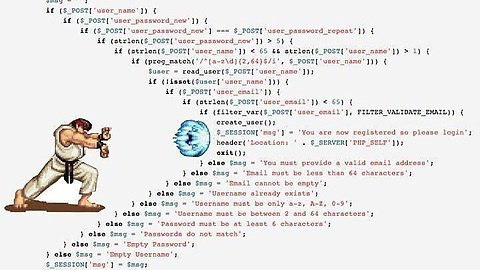
\includegraphics[height=0.7\paperheight]{ryu.jpg}
  \end{center}
\end{frame}


\begin{frame}{Lukier składniowy (\texttt{do}-notation):}
  \texttt{
    \ \ do result <- action \\
    \ \ \ \ \ \ actions  ... \\
  } \ \\ \pause
  przekształcamy do: \\ \pause
  \texttt{
    \ \ pass action (λ result -> do actions ...) \\
  } \ \\  \pause
  \ \\
  Uwaga: W Haskellu, \texttt{pass} zapisujemy jako
  \texttt{>>=} i wymawiamy ``bind''.
\end{frame}

\begin{frame}{Relacja pomiędzy \texttt{pass} a \texttt{<|}}
  \pause
  \texttt{pass$_m$ :: $m$ a -> (a -> $m$ b)} \\ \pause
  \texttt{<|$_m$ ::\ (b -> $m$ c) -> (a -> $m$ b) -> (a -> $m$ c)} \\ \pause
  \texttt{pass value function = (function <| id) value} \\ \pause
  \texttt{(f <| g) x = pass (g x) f} \\ \pause
  \texttt{return$_m$ :: (a -> $m$ a)} \\ \pause
  \texttt{return$_m$ = id$_m$}
\end{frame}

\begin{frame}
  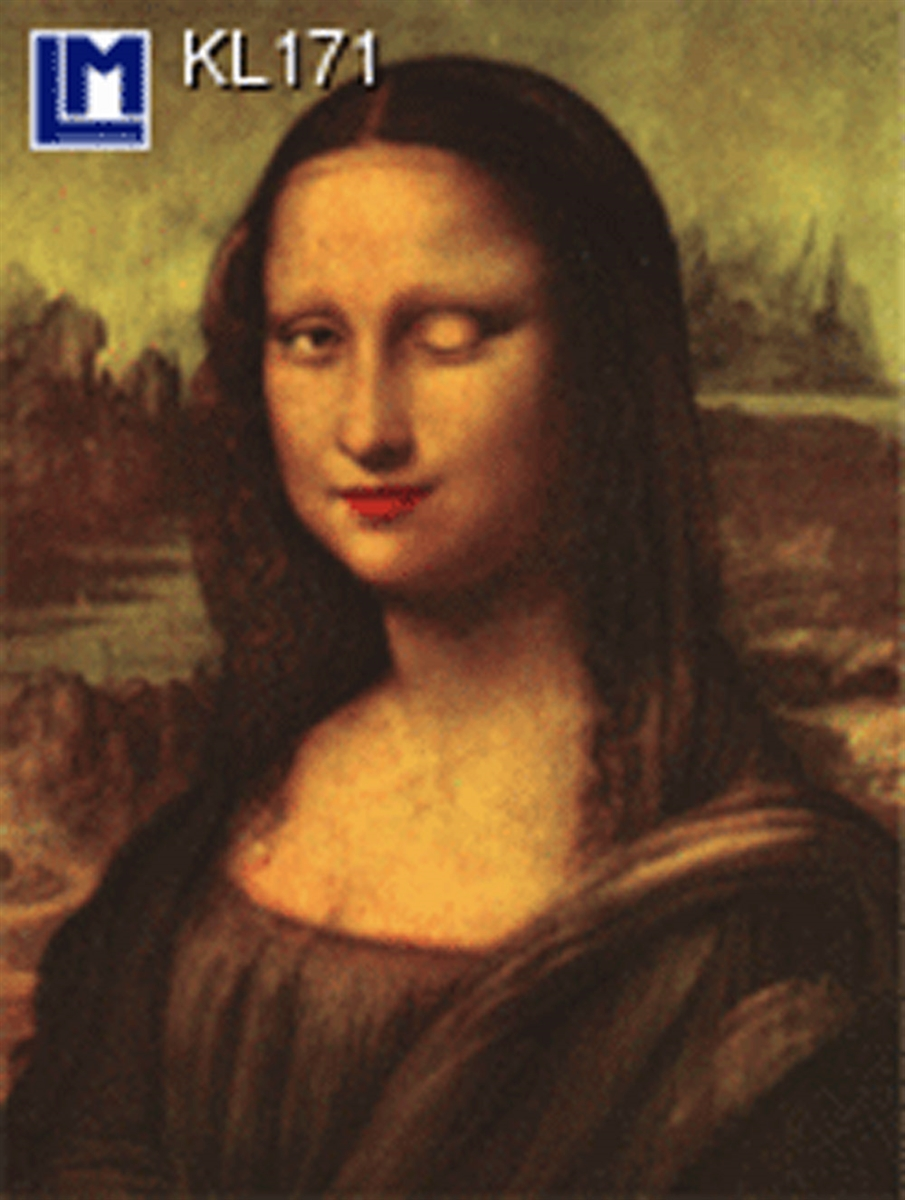
\includegraphics[height=\textheight]{monada.jpg}  
\end{frame}

\end{document}
